\chapter{Bildakquise und Datenaufbereitung}
Eine der grundlegenden Funktionalitäten des Projektes ist die Anzeige der Bilddaten des Ultraschallgerätes auf einem Smartphone Display. Dieser Prozess kann auf verschiedene Arten implementiert werden, welche unterschiedliche Vor- und Nachteile haben. Alle Ansätze haben jedoch eine grundlegende Abfolge von Arbeitsschritten gemein (siehe Abbildung \ref{fig:Bildakquise_schritte}).\\

\begin{figure}[h]
	\centering
	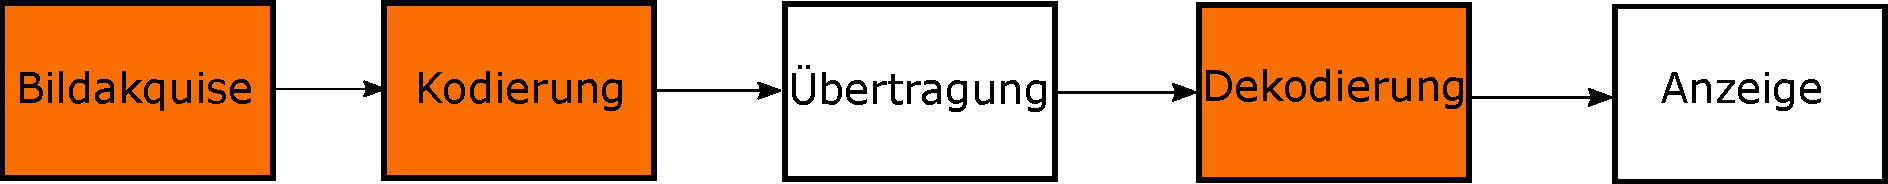
\includegraphics[width=1\textwidth]{Bilder/BildakquiseUndDatenaufbereitung/Bildakquise_schritte.pdf}
	\caption{Prozessschitte zur Anzeige der der Bilddaten auf dem Zielgerät. Die in diesem Kapitel behandelten Schritte sind farbig markiert.}
	\label{fig:Bildakquise_schritte}
\end{figure}

Im vorliegenden Kapitel wird primär auf die Schritte \textit{Bildakquise}, \textit{Kodierung} sowie \textit{Dekodierung} eingegangen, da die Implementierungen dieser Funktionalitäten direkt voneinander abhängen und somit nicht getrennt betrachtet werden können. Die Datenübertragung und Anzeige der Bilddaten bleiben hingegen unbeeinflusst von den genannten Prozessschritten und werden somit gesondert behandelt.\\

\section{Bildakquise}
Der Prozesschritt der Bildakquise beinhaltet die Ermittlung der Bilddaten von dem Quellgerät. Dabei können, je nach vorhandener Hard- und Softwarekonfiguration verschiedene Ansätze verfolgt werden.\\
\\
Ein möglicher Ansatz ist die Verwendung eines Hardwareadapters (\glqq FrameGrabber\grqq), welcher die Videosignale des Quellgerätes über dessen Videoausgang entgegennimmt und über eine Datenschnittstelle einem verarbeitenden Gerät zur Verfügung stellt. Ein Vorteil dieser Vorgehensweise ist die Simplizität in Bezug auf das Quellgerät. Da das Videosignal über bereits vorhandene, standardisierte Schnittstellen übertragen wird, muss keine Veränderung an der Software des Gerätes vorgenommen werden.\\
Im Gegenzug dazu wird jedoch ein weiteres Gerät, welches die Bilddaten entgegennimmt und verarbeitet, benötigt. Damit steigt die Gesamtkomplexität des Systems erheblich an, da statt einem Quell- und einem Zielgerät nunmehr ein Quellgerät, ein Zwischengerät zur Verarbeitung und ein Zielgerät benötigt werden.\\

\begin{figure}[h]
	\centering
	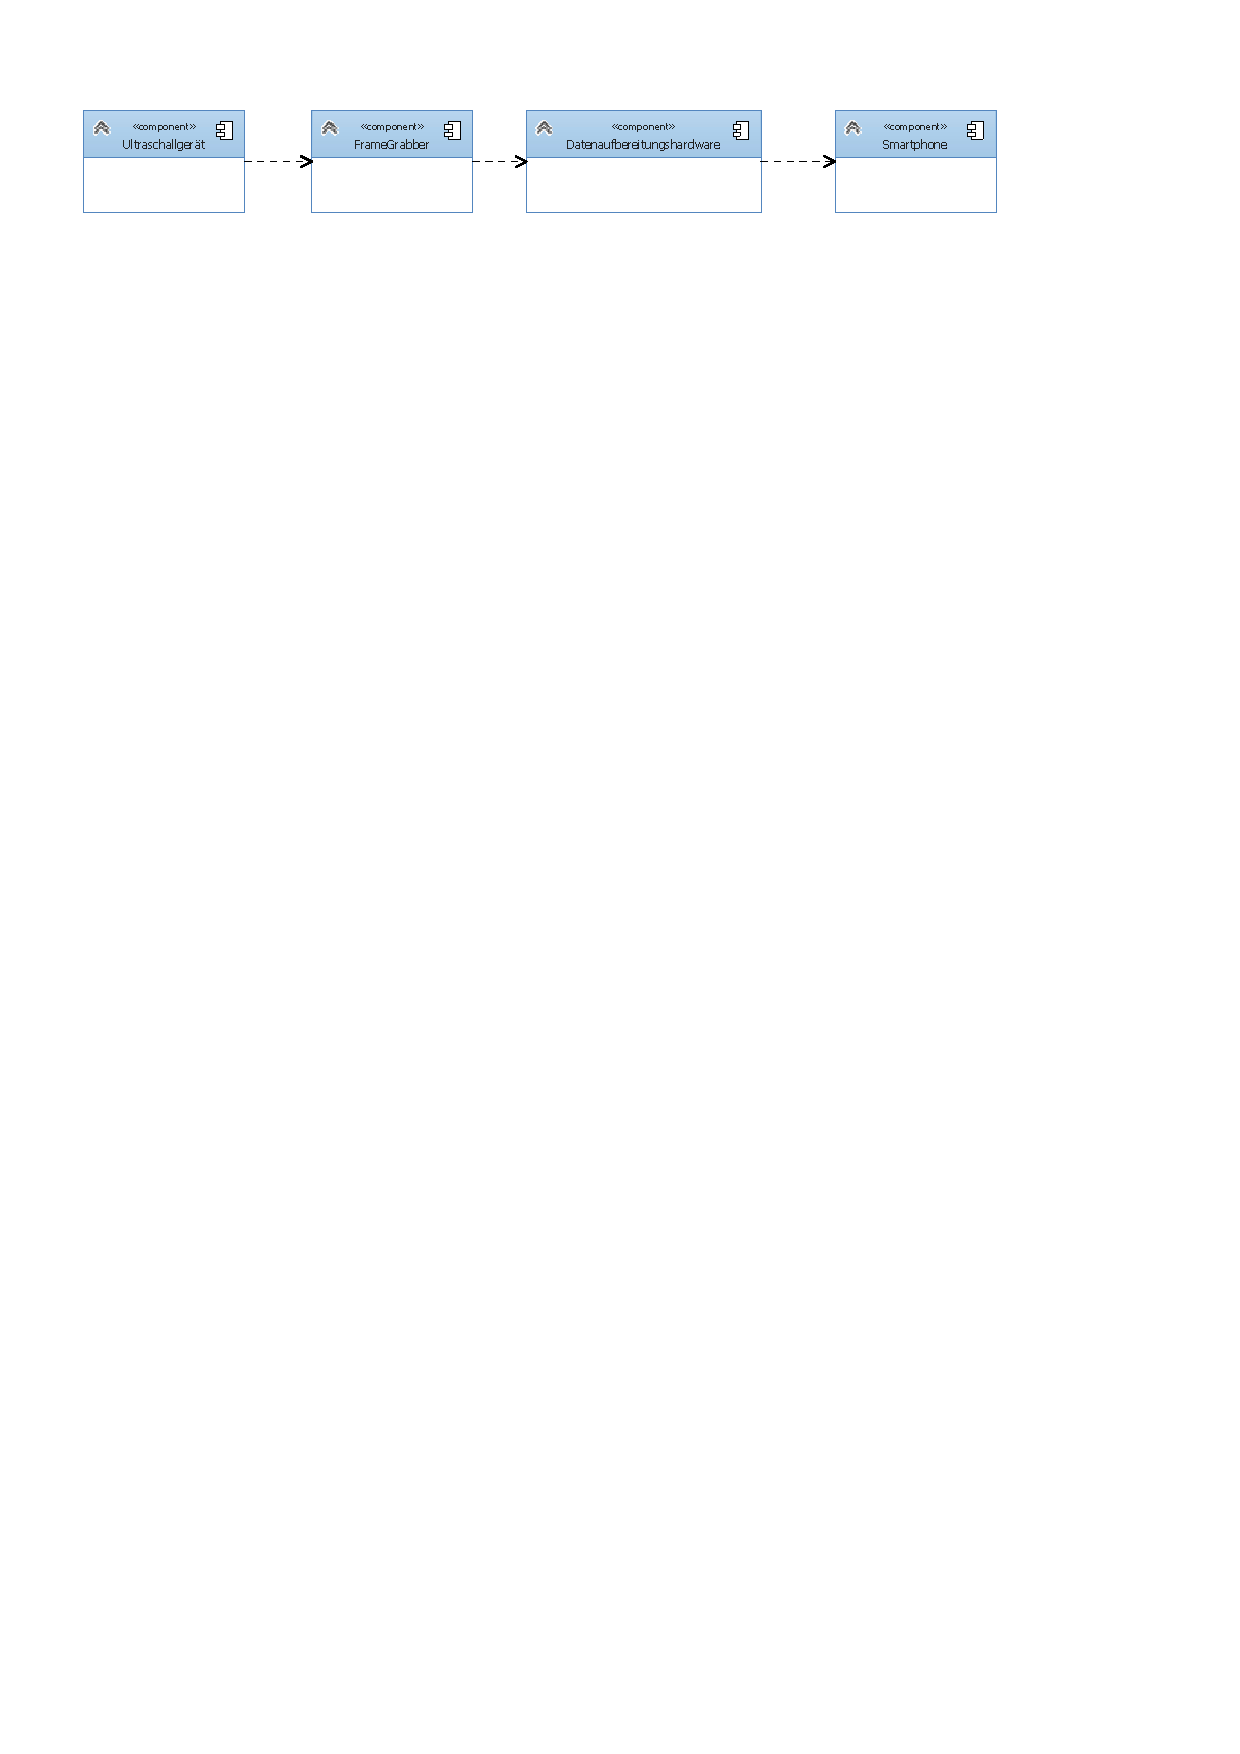
\includegraphics[width=1\textwidth]{Bilder/BildakquiseUndDatenaufbereitung/Bildakquise_ansatz1.pdf}
	\caption{Bildakquise mittels eines FrameGrabbers}
	\label{fig:Bildakquise_schritte}
\end{figure}

~\\
Statt der Nutzung eines FrameGrabbers zur Aufnahme der Bilddaten kann auch eine Software, welche die Daten direkt auf dem Ultraschallgerät  aufnimmt und aufbereitet, genutzt werden. Hierzu muss jedoch direkter Zugriff auf das Betriebssystem des Ultraschallgerätes erlangt werden, was sich bei proprietären, geschlossenen Systemen schwierig gestalten kann. Des Weiteren muss die Systemleistung des Quellgerätes ausreichen, um neben der eigentlichen Bildverarbeitung, welche für die Aufnahme des Ultraschallbildes durchgeführt wird, auch noch die Bildakquise und Datenaufbereitung durchzuführen.\\
Der Vorteil dieses Ansatzes im Vergleich zur Nutzung eines FrameGrabbers ist der Wegfall von zwei Hardwarekomponenten im Gesamtsystem: Der FrameGrabber und die Hardware zur Zwischenverarbeitung entfallen, da die entsprechenden Arbeitsschritte direkt auf dem Ultraschallgerät durchgeführt werden können.

\section{Kodierung}
Bei der Kodierung werden die zuvor aufgenommen Bilddaten aufbereitet, um die Übertragung über einen beliebigen Datenkanal zu erleichtern. Dies ist vor allem notwendig, da die Datenmenge der unbehandelten Bilddaten zu hoch für eine Übertragung mittels eines kabellosen Mediums ist.  Wird die Framerate\footnote{Framerate bezeichnet die Anzahl der angezeigten Bilder pro Sekunde} auf 30 FPS\footnote{Frames per second - Bilder pro Sekunde}, die Bildauflösung auf $1024*768$ Pixel und die Farbtiefe auf drei Bytes pro Pixel festgelegt, ergibt sich eine erforderliche Datenrate von
\begin{equation}
D_r=1024*768*3*30=67.5 MByte/s.
\end{equation}
Wenn als Übertragungsmedium WLAN genutzt wird und der 802.11ac\footcite{WIFIStandard} Standard vorausgesetzt werden kann, ist bei einer üblichen Kanalbreite von 20 MHz eine maximale Übertragunsgrate von $96.3 Mbit/s$ oder $12 MByte/s$ möglich. Folglich können die Daten nicht ohne vorherige Kompression übertragen werden.

\section{Dekodierung}
Die Dekodierung rekonstruiert aus dem übertragenen Datenstrom die ursprünglichen Frames und gibt sie an zur Weiterverarbeitung und Anzeige frei. Dieser Prozessschritt wird auf dem Smartphone durchgeführt, da er erst nach der Datenübertragung stattfinden kann.

\section{Implementierung mit FFmpeg}
Im Verlaufe des Projektes wurden zwei verschiedene Ansätze implementiert und getestet. Bei dem ersten Ansatz wurden die Schritte der Bildakquise und Kodierung unter Zuhilfenahme der FFmpeg-Bibliothek\footcite{FFmpeg} realisiert, während zur Dekodierung unter anderem die Android MediaCodec Api\footcite{AndroidMediaCodec} genutzt wurde.\\
Die FFmpeg-Bibliothek bietet die Möglichkeit, über einen Kommandozeilenbefehl den aktuellen Bildschirminhalt als Videostream abzugreifen sowie die entstehenden Daten mit diversen Videocodecs zu kodieren. Der resultierende Datenstrom kann über die unter Linux vorhandene Pipe-Funktionalität in einen gesonderten Prozess umgeleitet werden, welcher die Übertragung bewerkstelligt.
